\documentclass[11pt,a4paper,twoside]{book}

% --- Paquetes Básicos y Tipografía ---
\usepackage[utf8]{inputenc}
\usepackage[T1]{fontenc}
\usepackage[spanish,es-tabla]{babel}
\usepackage{lmodern}
\usepackage{microtype}
\usepackage{eurosym}

% --- Geometría de Página (Estándar Encuadernación ETSII UPM) ---
\usepackage[
    a4paper,
    top=30mm,
    bottom=30mm,
    inner=30mm,
    outer=25mm,
    headheight=16pt
]{geometry}

% --- Matemáticas, Tablas y Gráficos ---
\usepackage{amsmath,amssymb,amsfonts}
\usepackage{graphicx}
\usepackage{booktabs}
\usepackage{array}
\usepackage{multirow}
\usepackage{float}
\usepackage{caption}
\usepackage{subcaption}

% --- Enlaces y URLs ---
\usepackage{xcolor}
\definecolor{upmblue}{RGB}{0, 75, 141}
\usepackage{hyperref}
\hypersetup{
    colorlinks=true,
    linkcolor=upmblue,
    citecolor=upmblue,
    urlcolor=upmblue
}

% --- Código Fuente ---
\usepackage{listings}
\lstset{
    basicstyle=\ttfamily\footnotesize,
    breaklines=true,
    frame=single,
    rulecolor=\color{gray!40},
    numbers=left,
    numberstyle=\tiny\color{gray},
    keywordstyle=\color{upmblue}\bfseries,
    stringstyle=\color{teal},
    commentstyle=\color{gray}\itshape
}

% --- Encabezados y Pies de Página ---
\usepackage{fancyhdr}
\pagestyle{fancy}
\fancyhf{}
\fancyhead[LE,RO]{\thepage}
\fancyhead[RE]{\nouppercase{\leftmark}}
\fancyhead[LO]{\nouppercase{\rightmark}}
\renewcommand{\headrulewidth}{0.4pt}

% ====================================================================
% DATOS DEL TRABAJO FIN DE MÁSTER (ETSII - UPM)
% ====================================================================
\newcommand{\tfmTitulo}{Orquestador de Misiones y Control Reactivo Multi-Robot mediante Behavior Trees para la Brigada de Búsqueda y Rescate RASTREO}
\newcommand{\tfmAutor}{Álvaro Pérez-Borbujo Mohedo}
\newcommand{\tfmDirector}{Dr. Christyan Cruz Ulloa}
\newcommand{\tfmPonente}{}
\newcommand{\tfmMaster}{Máster Universitario en Automática y Robótica (MUAR)}
\newcommand{\tfmDepartamento}{Departamento de Automática, Ingeniería Eléctrica y Electrónica e Informática Industrial (DISAM)}
\newcommand{\tfmCentro}{Centro de Automática y Robótica (CAR CSIC-UPM)}
\newcommand{\tfmFecha}{Madrid, 2026}

\begin{document}

% --- Páginas Preliminares (Roman) ---
\frontmatter

% Portada (Esquema provisional ETSII UPM)
\begin{titlepage}
    \centering
    {\scshape\LARGE Universidad Politécnica de Madrid \par}
    \vspace{0.3cm}
    {\scshape\Large Escuela Técnica Superior de Ingenieros Industriales \par}
    \vspace{1.5cm}
    
    % Logo UPM / ETSII (Placeholder)
    % \includegraphics[width=0.35\textwidth]{figuras/logo_etsii_upm.png}\par
    \vspace{1.5cm}
    
    {\Large\textbf{TRABAJO FIN DE MÁSTER}\par}
    \vspace{0.5cm}
    {\large \tfmMaster \par}
    \vspace{1.5cm}
    
    {\Huge\bfseries\color{upmblue} \tfmTitulo \par}
    \vspace{2cm}
    
    \begin{flushright}
        \textbf{Autor:} \tfmAutor \\
        \textbf{Director:} \tfmDirector \\
        \textbf{Centro:} \tfmCentro \\
        \textbf{Departamento:} \tfmDepartamento
    \end{flushright}
    
    \vfill
    {\large \tfmFecha \par}
\end{titlepage}

% Índices
\tableofcontents
\listoffigures
\listoftables

% --- Cuerpo Principal (Arabic) ---
\mainmatter

\chapter{Introducción y Objetivos}
\label{chap:introduccion}

\section{Contexto y motivación}
\label{sec:contexto}

Las operaciones de búsqueda y rescate en estructuras colapsadas (\textit{Urban Search and Rescue}, USAR) tras desastres naturales o colapsos estructurales entrañan un riesgo crítico para los equipos de rescate humanos y las unidades caninas tradicionales. En estos entornos altamente confinados y dinámicos, la introducción de plataformas robóticas móviles capaces de explorar, evaluar la estabilidad del terreno y localizar a víctimas de manera autónoma representa un salto cualitativo fundamental.

El presente Trabajo Fin de Máster se enmarca en las actividades de investigación desarrolladas en el **Centro de Automática y Robótica (CAR CSIC-UPM)** en el contexto del proyecto \textbf{RASTREO} (\textit{«Brigada Robotizada de Rastreo Canino y Asistencia Humanoide para respuesta inteligente en Búsqueda y Rescate»}).

\section{Objetivos del trabajo}
\label{sec:objetivos}

El objetivo general de este proyecto es el diseño, desarrollo e integración de un sistema de control reactivo y orquestación para una brigada homogénea de tres robots cuadrúpedos, permitiendo la asignación y ejecución distribuida de misiones en entornos desafiantes.

Para alcanzar dicho objetivo general, se establecen los siguientes \textbf{objetivos específicos}:

\begin{enumerate}
    \item \textbf{Controlador de comunicaciones en bajo nivel (C++20):} Desarrollar un driver serie robusto, de alta eficiencia y determinista para la interacción directa con el microcontrolador de los robots XGO Mini 2S.
    \item \textbf{Arquitectura de despliegue modular:} Diseñar una infraestructura basada en microservicios contenerizados mediante Docker sobre ROS 2 Jazzy, garantizando aislamiento de fallos entre la navegación y el hardware.
    \item \textbf{Integración de navegación autónoma local:} Desplegar la pila de navegación Nav2 con el controlador local omnidireccional MPPI, adaptado a la cinemática de las plataformas cuadrúpedas.
    \item \textbf{Control reactivo individual tolerante a fallos:} Diseñar e implementar árboles de comportamiento (\textit{Behavior Trees}) mediante la librería \texttt{BehaviorTree.CPP v4}, estructurando de forma jerárquica la respuesta ante contingencias y fallos críticos.
    \item \textbf{Orquestador de misiones multi-robot:} Desarrollar un despachador global en C++20 que asigne dinámicamente misiones operativas a la brigada (exploración, barrido sistemático, tendido de cable guía, marcaje de víctimas y relevo de batería).
    \item \textbf{Validación experimental en simulación y hardware:} Evaluar el rendimiento del sistema mediante pruebas en lazo cerrado en simulación (SIL) y contrastar la fiabilidad del driver en los robots físicos.
\end{enumerate}

\section{Estructura del documento}
\label{sec:estructura}

La memoria se organiza en ocho capítulos estructurados de forma secuencial: el Capítulo~\ref{chap:investigacion} expone la plataforma de hardware y el estado del arte; el Capítulo~\ref{chap:arquitectura} detalla la arquitectura de software y el driver C++20; el Capítulo~\ref{chap:behavior_trees} aborda la metodología y diseño de los \textit{Behavior Trees}; el Capítulo~\ref{chap:orquestador} describe el orquestador global de la flota; el Capítulo~\ref{chap:pruebas} presenta los resultados experimentales y benchmarks; el Capítulo~\ref{chap:presupuesto} recoge el presupuesto y planificación del proyecto; y el Capítulo~\ref{chap:conclusiones} resume las conclusiones y líneas futuras.

\chapter{Investigación previa y plataforma robótica}
\label{chap:investigacion}

En este capítulo se describe la plataforma de hardware utilizada para la brigada de búsqueda y rescate, las especificaciones sensoriales de las unidades, el software original proporcionado por el fabricante y la justificación técnica que motivó el desarrollo de un controlador nativo en C++20.

\section{Plataforma física: Flota de cuadrúpedos XGO Mini 2S}
\label{sec:perros}

El proyecto se sustenta sobre una flota homogénea compuesta por \textbf{tres robots cuadrúpedos idénticos} del modelo \textit{XGO Mini 2S}, desarrollados por \textit{Luwu Dynamics} (\url{https://wiki.xgorobot.com/kb/the-xgo-series-robot/cmpidwcrq000jhjqr5awou1iy}). 

Cada una de las tres unidades cuenta con la siguiente configuración física y sensorial:

\subsection{Unidad de procesamiento a bordo}
\begin{itemize}
    \item \textbf{Computador de a bordo:} Raspberry Pi Compute Module 5 Lite (CM5). Este módulo centraliza las tareas de percepción, localización y toma de decisiones a bordo, operando como nodo de cómputo en el borde (\textit{Edge Computing}).
\end{itemize}

\subsection{Sensores cinemáticos e inerciales}
\begin{itemize}
    \item \textbf{Unidad de Medición Inercial (IMU):} Sensor de 6 grados de libertad (giróscopo de 3 ejes y acelerómetro de 3 ejes), imprescindible para la detección de desniveles, estimación de actitud y detección de vuelcos.
    \item \textbf{Sensores de posición articular:} Encoders integrados en los servomotores de las cuatro extremidades para el control cinemático de bajo nivel.
\end{itemize}

\subsection{Sensor LiDAR 2D}
Para la construcción de mapas métricos y la evasión reactiva de obstáculos, cada robot dispone de un sensor LiDAR 2D montado sobre el chasis superior. Sus especificaciones técnicas detalladas se resumen en la Tabla~\ref{tab:especificaciones_lidar}.

\begin{table}[htbp]
    \centering
    \caption{Especificaciones técnicas del sensor LiDAR embarcado en los robots XGO Mini 2S.}
    \label{tab:especificaciones_lidar}
    \begin{tabular}{p{5.5cm} p{3.5cm} p{5.5cm}}
        \toprule
        \textbf{Parámetro} & \textbf{Valor} & \textbf{Notas} \\
        \midrule
        Radio de alcance (\textit{Ranging Radius}) & 0.05 -- 12\,m & @80\% reflectividad; 0.05 -- 4\,m @10\% reflectividad \\
        Precisión de medida & $\pm 20$\,mm & Error sistemático en rango completo \\
        Frecuencia de escaneo & 6 -- 12\,Hz & Ajustable por software (defecto 6\,Hz) \\
        Frecuencia de muestreo & 4000\,Hz & Tasa de adquisición angular \\
        Ángulo de escaneo & $360^\circ$ & Cobertura omnidireccional en el plano \\
        Resistencia a luz ambiental & 60000\,Lux & Inmunidad frente a fuentes de luz externa \\
        Resolución angular & $0.54^\circ$ & Discretización angular por muestra \\
        Seguridad láser & FDA Class I & Inocuo para la vista (\textit{Eye safe}) \\
        Voltaje de alimentación & 4.8\,V -- 5.2\,V & Típico 5.0\,V \\
        Interfaz de comunicación & UART / GH1.25-4P & Protocolo serie asíncrono \\
        Dimensiones & $38.6 \times 38.6 \times 33.9$\,mm & Formato compacto \\
        Peso & Aprox. 45\,g & Carga útil mínima sobre el robot \\
        \bottomrule
    \end{tabular}
\end{table}

\subsection{Carga útil adicional: Brazo robótico}
Las tres unidades van equipadas con el **brazo robótico articulado con pinza (\textit{gripper})** oficial de Luwu Dynamics. Este actuador dota a cada cuadrúpedo de capacidad de manipulación física en el entorno, permitiendo ejecutar tareas de agarre, despeje de pequeños obstáculos o el despliegue del carrete de cable guía (Misión M5 del proyecto RASTREO).

---

\section{El SDK original del fabricante y análisis del software base}
\label{sec:sdk}

El fabricante proporciona una distribución de sistema operativo basada en Raspberry Pi OS junto con un manual de referencia (\url{https://wiki.xgorobot.com/kb/the-xgo-series-robot/cmqcbgk9800178ffsqm8jseze}). La capa de comunicación oficial provista por Luwu Dynamics se basa en una librería interpretada en Python (\texttt{xgolib\_dog.py}), la cual interactúa con la placa controladora de bajo nivel del perro a través del puerto serie UART (\texttt{/dev/ttyAMA0}).

\section{Justificación técnica del desarrollo del nuevo driver C++20}
\label{sec:justificacion_cpp}

Si bien el SDK original en Python resulta funcional para demostraciones básicas y teleoperación elemental, en este trabajo se optó por rediseñar e implementar un controlador de comunicaciones completamente nuevo en \textbf{C++20 moderno} (\texttt{xgo\_driver\_cpp}). 

Esta decisión técnica se fundamenta en los siguientes aspectos:

\begin{enumerate}
    \item \textbf{Optimización de recursos en la Raspberry Pi CM5:} En un escenario de rescate real, el computador de a bordo debe ejecutar de forma simultánea algoritmos computacionalmente intensivos (SLAM con \texttt{slam\_toolbox}, planificación y seguimiento de trayectorias locales mediante \texttt{Nav2 MPPI}, y el motor de toma de decisiones de \textit{Behavior Trees}). Destinar ciclos de CPU a un intérprete de Python para la comunicación serie básica limita la capacidad de respuesta de los lazos de control más críticos.
    \item \textbf{Eliminación del Global Interpreter Lock (GIL) y determinismo temporal:} El driver en C++20 implementa un decodificador de tramas mediante una máquina de estados finitos (FSM) de cero copias y gestión RAII de los descriptores de archivo serie (\texttt{termios}), garantizando tiempos de lectura y escritura deterministas.
    \item \textbf{Integración nativa con la pila ROS 2:} Al programar el driver en C++20, se evitan capas intermedias de conversión de tipos de datos o bindings mixtos, facilitando la publicación directa de mensajes estandarizados (\texttt{nav\_msgs/msg/Odometry}, \texttt{sensor\_msgs/msg/Imu}, \texttt{sensor\_msgs/msg/BatteryState}).
    \item \textbf{Rendimiento computacional contrastado:} Los ensayos de rendimiento realizados sobre 1.000.000 de operaciones demostraron una aceleración global de más de 20 veces respecto a la librería original del fabricante (destacando una mejora de hasta 340 veces en el desempaquetado de datos numéricos en coma flotante), situando el consumo medio de CPU del driver por debajo del 0.5\%.
\end{enumerate}

---

\section{Estado de validación experimental actual}
\label{sec:estado_validacion}

Para mantener la rigurosidad y trazabilidad en la memoria del trabajo, se delimita el grado de validación empírica alcanzado en cada capa del sistema:

\begin{itemize}
    \item \textbf{Capa de bajo nivel (Driver C++20):} Validada experimentalmente en hardware físico real. Se ha comprobado con éxito la transmisión bidireccional por puerto serie UART a 115200 baudios, la emisión de comandos de locomoción y la recepción e interpretación de la telemetría del robot.
    \item \textbf{Capa de navegación y ROS 2 (Nav2 y Behavior Trees):} Desarrollada a nivel de arquitectura y paquetes software, y validada preliminarmente mediante herramientas de simulación (modelo cinemático en Gazebo y entorno SIL con emulador de hardware serie \textit{Mock MCU}). Las pruebas de navegación autónoma integrada con Nav2 sobre los perros físicos en el entorno de pruebas constituyen la siguiente fase experimental del proyecto.
\end{itemize}

\chapter{Arquitectura Software del Sistema}
\label{chap:arquitectura}

En este capítulo se describe el diseño modular de la pila de software embarcada en los cuadrúpedos, el despliegue en microservicios contenerizados y los fundamentos del controlador de bajo nivel en C++20.

\section{Arquitectura en microservicios desacoplados (Docker)}
\label{sec:docker_arch}

Para evitar que un bloqueo en los algoritmos de navegación o SLAM comprometa la estabilidad y seguridad física del robot, el sistema se estructura en tres contenedores Docker independientes que comparten la red local del host (\texttt{Host Network}) sobre ROS 2 Jazzy:

\begin{enumerate}
    \item \textbf{\texttt{xgo\_driver}:} Contenedor dedicado al driver de comunicaciones en tiempo real en C++20. Gestiona el puerto serie físico (\texttt{/dev/ttyAMA0}), un temporizador de seguridad (\textit{watchdog} de 0.5\,s) y publica la odometría, telemetría de batería y datos de la IMU.
    \item \textbf{\texttt{xgo\_nav}:} Contenedor de la pila de navegación Nav2, configurado con el controlador predictivo omnidireccional MPPI (\textit{Model Predictive Path Integral}), localización probabilística AMCL y mapas de costes estáticos y dinámicos.
    \item \textbf{\texttt{xgo\_mock\_mcu}:} Emulador virtual del microcontrolador de bajo nivel para pruebas en lazo cerrado (\textit{Software-in-the-Loop}, SIL), permitiendo simular las respuestas del robot sobre un pseudoterminal sin necesidad del hardware físico.
\end{enumerate}

\section{Controlador de bajo nivel: \texttt{xgo\_driver\_cpp}}
\label{sec:driver_cpp}

El paquete \texttt{xgo\_driver\_cpp} sustituye a la librería en Python original proporcionando comunicación serie asíncrona mediante el estándar POSIX \texttt{termios} (modo raw 8N1). Sus características principales incluyen:

\begin{itemize}
    \item \textbf{Máquina de estados finitos (FSM):} Decodificación continua de paquetes entrantes tolerante a ruido e interferencias en la línea UART.
    \item \textbf{Gestión de recursos mediante RAII:} Adquisición y cierre determinista de los descriptores de archivo serie, previniendo fugas de memoria o puertos bloqueados.
    \item \textbf{Parada segura automática:} Incorporación de un watchdog hardware/software que comanda velocidad nula a los servomotores si se interrumpe la emisión de consignas durante más de 500\,ms.
\end{itemize}

\section{Entorno de simulación y emulador SIL}
\label{sec:simulacion_mock}

\textit{[Sección esquemática: Descripción del modelo URDF en Gazebo/RViz2 y de la interfaz del emulador Mock MCU con cuadro de mando ASCII para validación preliminar en local].}

\chapter{Control Reactivo Individual mediante Behavior Trees}
\label{chap:behavior_trees}

En este capítulo se formaliza la toma de decisiones autónoma y la respuesta reactiva a fallos en cada cuadrúpedo mediante árboles de comportamiento (\textit{Behavior Trees}), empleando el estándar de la industria \texttt{BehaviorTree.CPP v4}.

\section{Metodología de diseño en cinco fases}
\label{sec:metodologia_bt}

El diseño del árbol de comportamiento se articula siguiendo una metodología descendente (\textit{Top-Down}) en cinco fases:

\begin{enumerate}
    \item \textbf{Fase 1: Análisis de escenarios y modos de fallo.} Identificación del camino nominal (\textit{Happy Path}) y clasificación de las contingencias operativas (U1 a U9: caídas, desconexión Wi-Fi, batería baja, parada de emergencia, etc.).
    \item \textbf{Fase 2: Catálogo de nodos hoja y contrato del Blackboard.} Definición estricta de las Condiciones (de solo lectura), Acciones (asíncronas con duración) y variables compartidas tipadas.
    \item \textbf{Fase 3: Estructuración Top-Down y priorización.} Ordenación jerárquica de izquierda a derecha (Seguridad $\rightarrow$ Batería $\rightarrow$ Enlace Wi-Fi $\rightarrow$ Despacho de misión $\rightarrow$ Reposo), delegando eventos sensoriales de víctima al orquestador.
    \item \textbf{Fase 4: Modelado visual XML (Groot2).} Creación de la descripción estandarizada en formato XML (\texttt{BehaviorTree.CPP v4}) con definición de subárboles modulares y catálogo de tipos para validación visual previa.
    \item \textbf{Fase 5: Implementación C++20.} Programación modular de las clases C++ especializadas conectadas a los tópicos y acciones de ROS 2.
\end{enumerate}

\section{Catálogo de misiones operativas (M1 a M6)}
\label{sec:catalogo_misiones}

El árbol de cada robot cuadrúpedo es capaz de ejecutar seis misiones operativas asignadas por el orquestador global:
\begin{itemize}
    \item \textbf{M1: Exploración activa de mapa desconocido} (Active SLAM con \texttt{slam\_toolbox}).
    \item \textbf{M2: Barrido sistemático en mapa conocido} (Cobertura coordinada de áreas libres).
    \item \textbf{M3: Despacho multi-punto óptimo} (Navegación punto a punto evitando colisiones mutuas).
    \item \textbf{M4: Marcaje y balizamiento de víctima} (Triangulación y transmisión de pose segura).
    \item \textbf{M5: Despliegue de cable guía físico} (Accionamiento de brazo y tendido de línea de vida).
    \item \textbf{M6: Relevo dinámico de batería y retorno a base} (Evacuación de unidades en descarga crítica).
\end{itemize}

\section{Estructura interna del despachador de tareas}
\label{sec:task_dispatcher}

\textit{[Sección esquemática: Detalle de la rama selectora de subárboles mediante la variable \texttt{task\_type} del Blackboard y condiciones \texttt{IsTaskType} para ejecución aislada de cada misión].}

\chapter{Orquestador y Coordinación de Flota Multi-Robot}
\label{chap:orquestador}

\section{Arquitectura del orquestador central en C++20}
\label{sec:orquestador_c20}

El orquestador de flota actúa como el puesto de mando centralizado que supervisa el estado global de la brigada de rescate. Diseñado en C++20, centraliza la recepción de telemetría de los tres cuadrúpedos y gestiona la asignación óptima de misiones.

\section{Mecanismo de despacho de órdenes (ROS 2 Actions)}
\label{sec:despacho_ordenes}

La interacción entre el orquestador global y los árboles de comportamiento individuales se implementa mediante interfaces de acción estándar de ROS 2 (\texttt{ExecuteTask.action}):
\begin{itemize}
    \item \textbf{Meta (\textit{Goal}):} Identificador de la tarea, tipo de misión (\texttt{task\_type}) y datos geométricos (objetivo o lista de waypoints).
    \item \textbf{Retroalimentación (\textit{Feedback}):} Porcentaje de avance, posición instantánea del robot y estado de salud operativa.
    \item \textbf{Resultado (\textit{Result}):} Confirmación de éxito (\texttt{SUCCESS}), aborto por contingencia o reporte de causas de fallo.
\end{itemize}

\section{Sincronización y prevención de conflictos entre agentes}
\label{sec:sincronizacion_agentes}

\textit{[Sección esquemática: Reglas de prioridad para evitar bloqueos mutuos en pasillos y coordinación para misiones de relevo y marcaje cooperativo].}

\chapter{Pruebas Experimentales y Resultados}
\label{chap:pruebas}

En este capítulo se recogen los ensayos experimentales llevados a cabo tanto a nivel de emulación en software (\textit{Software-in-the-Loop}, SIL) como en la comunicación física sobre hardware (\textit{Hardware-in-the-Loop}, HIL).

\section{Evaluación del rendimiento computacional (Benchmark C++20 vs Python)}
\label{sec:benchmark_rendimiento}

Para cuantificar objetivamente la ganancia de rendimiento obtenida tras la reingeniería del driver, se ejecutó un banco de pruebas comparativo de 1.000.000 de operaciones consecutivas frente a la librería original en Python (\texttt{xgolib\_dog.py}) suministrada por el fabricante.

Los resultados empíricos obtenidos se detallan en la Tabla~\ref{tab:benchmark_driver}.

\begin{table}[htbp]
    \centering
    \caption{Comparativa de rendimiento entre la librería original Python y el nuevo driver C++20 (1.000.000 operaciones).}
    \label{tab:benchmark_driver}
    \begin{tabular}{lccc}
        \toprule
        \textbf{Operación evaluada} & \textbf{Python (\texttt{xgolib\_dog})} & \textbf{C++20 (\texttt{xgo\_driver})} & \textbf{Aceleración (\textit{Speedup})} \\
        \midrule
        Mapeo físico y creación trama TX & 440.74\,ms & 30.06\,ms & \textbf{14.6$\times$} \\
        Desempaquetado flotante (\texttt{Byte2float}) & 285.68\,ms & 0.84\,ms & \textbf{340$\times$} \\
        Parseo de flujo UART RX (900.000 bytes) & 54.29\,ms & 7.17\,ms & \textbf{7.6$\times$} \\
        \midrule
        \textbf{Tiempo total de ejecución} & \textbf{780.71\,ms} & \textbf{38.08\,ms} & \textbf{20.5$\times$ más rápido} \\
        \bottomrule
    \end{tabular}
\end{table}

Como se observa, el nuevo controlador reduce el tiempo total de procesamiento en más de un 95\%, con una mejora crítica en el desempaquetado numérico de telemetría de 340 veces, liberando capacidad computacional esencial en la Raspberry Pi CM5.

\section{Validación en hardware físico real}
\label{sec:validacion_hw}

Se ha verificado experimentalmente el enlace serie bidireccional entre la Raspberry Pi CM5 y la placa controladora de los cuadrúpedos a través de \texttt{/dev/ttyAMA0}. Las pruebas confirman la recepción continua de la IMU y la odometría de los servomotores a 115200 baudios, así como la actuación correcta del mecanismo de parada por timeout del watchdog.

\section{Validación en simulación (SIL) sobre Gazebo Harmonic}
\label{sec:validacion_sil}

Para validar el comportamiento integral de la brigada multi-robot sin depender del emulador ligero de MCU, se ha ejecutado una batería automatizada de ocho pruebas de integración (\texttt{scripts/test\_bt\_gazebo.py}) sobre \textbf{Gazebo Harmonic} con tres cuadrúpedos \textit{XGO Mini 2S} operando simultáneamente en namespaces aislados (\texttt{/robot1}, \texttt{/robot2}, \texttt{/robot3}), puente \texttt{ros\_gz\_bridge} y tres instancias independientes del ejecutor \texttt{BehaviorTree.CPP~v4} (\texttt{bt\_executor\_node}) con registro de trazas \texttt{.btlog} para Groot2.

El objetivo de esta batería es verificar en bucle cerrado las cinco ramas prioritarias del árbol reactivo \texttt{rastreo\_bt.xml}: seguridad crítica (Rama~1), contingencia energética (Rama~2), pérdida de enlace Wi-Fi (Rama~3), despacho concurrente de misiones M2/M3/M6 (Rama~4) y reposo seguro (Rama~5). La Tabla~\ref{tab:resultados_sil_gazebo} resume los resultados obtenidos.

\begin{figure}[htbp]
    \centering
    \begin{subfigure}[b]{0.48\textwidth}
        \centering
        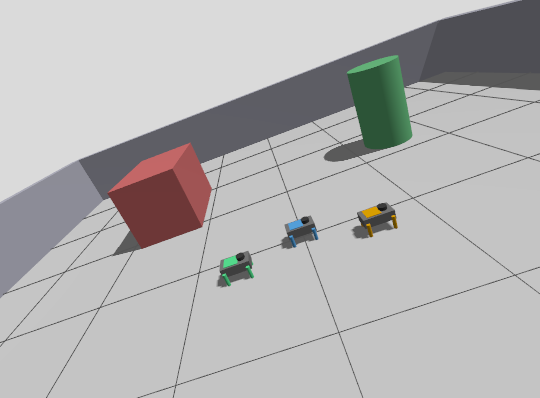
\includegraphics[width=\textwidth]{figuras/gazebo_fleet_3d.png}
        \caption{Escena 3D en Gazebo Harmonic (\texttt{room.sdf}) con R1 (naranja), R2 (azul) y R3 (verde).}
        \label{fig:gazebo_fleet_3d}
    \end{subfigure}
    \hfill
    \begin{subfigure}[b]{0.48\textwidth}
        \centering
        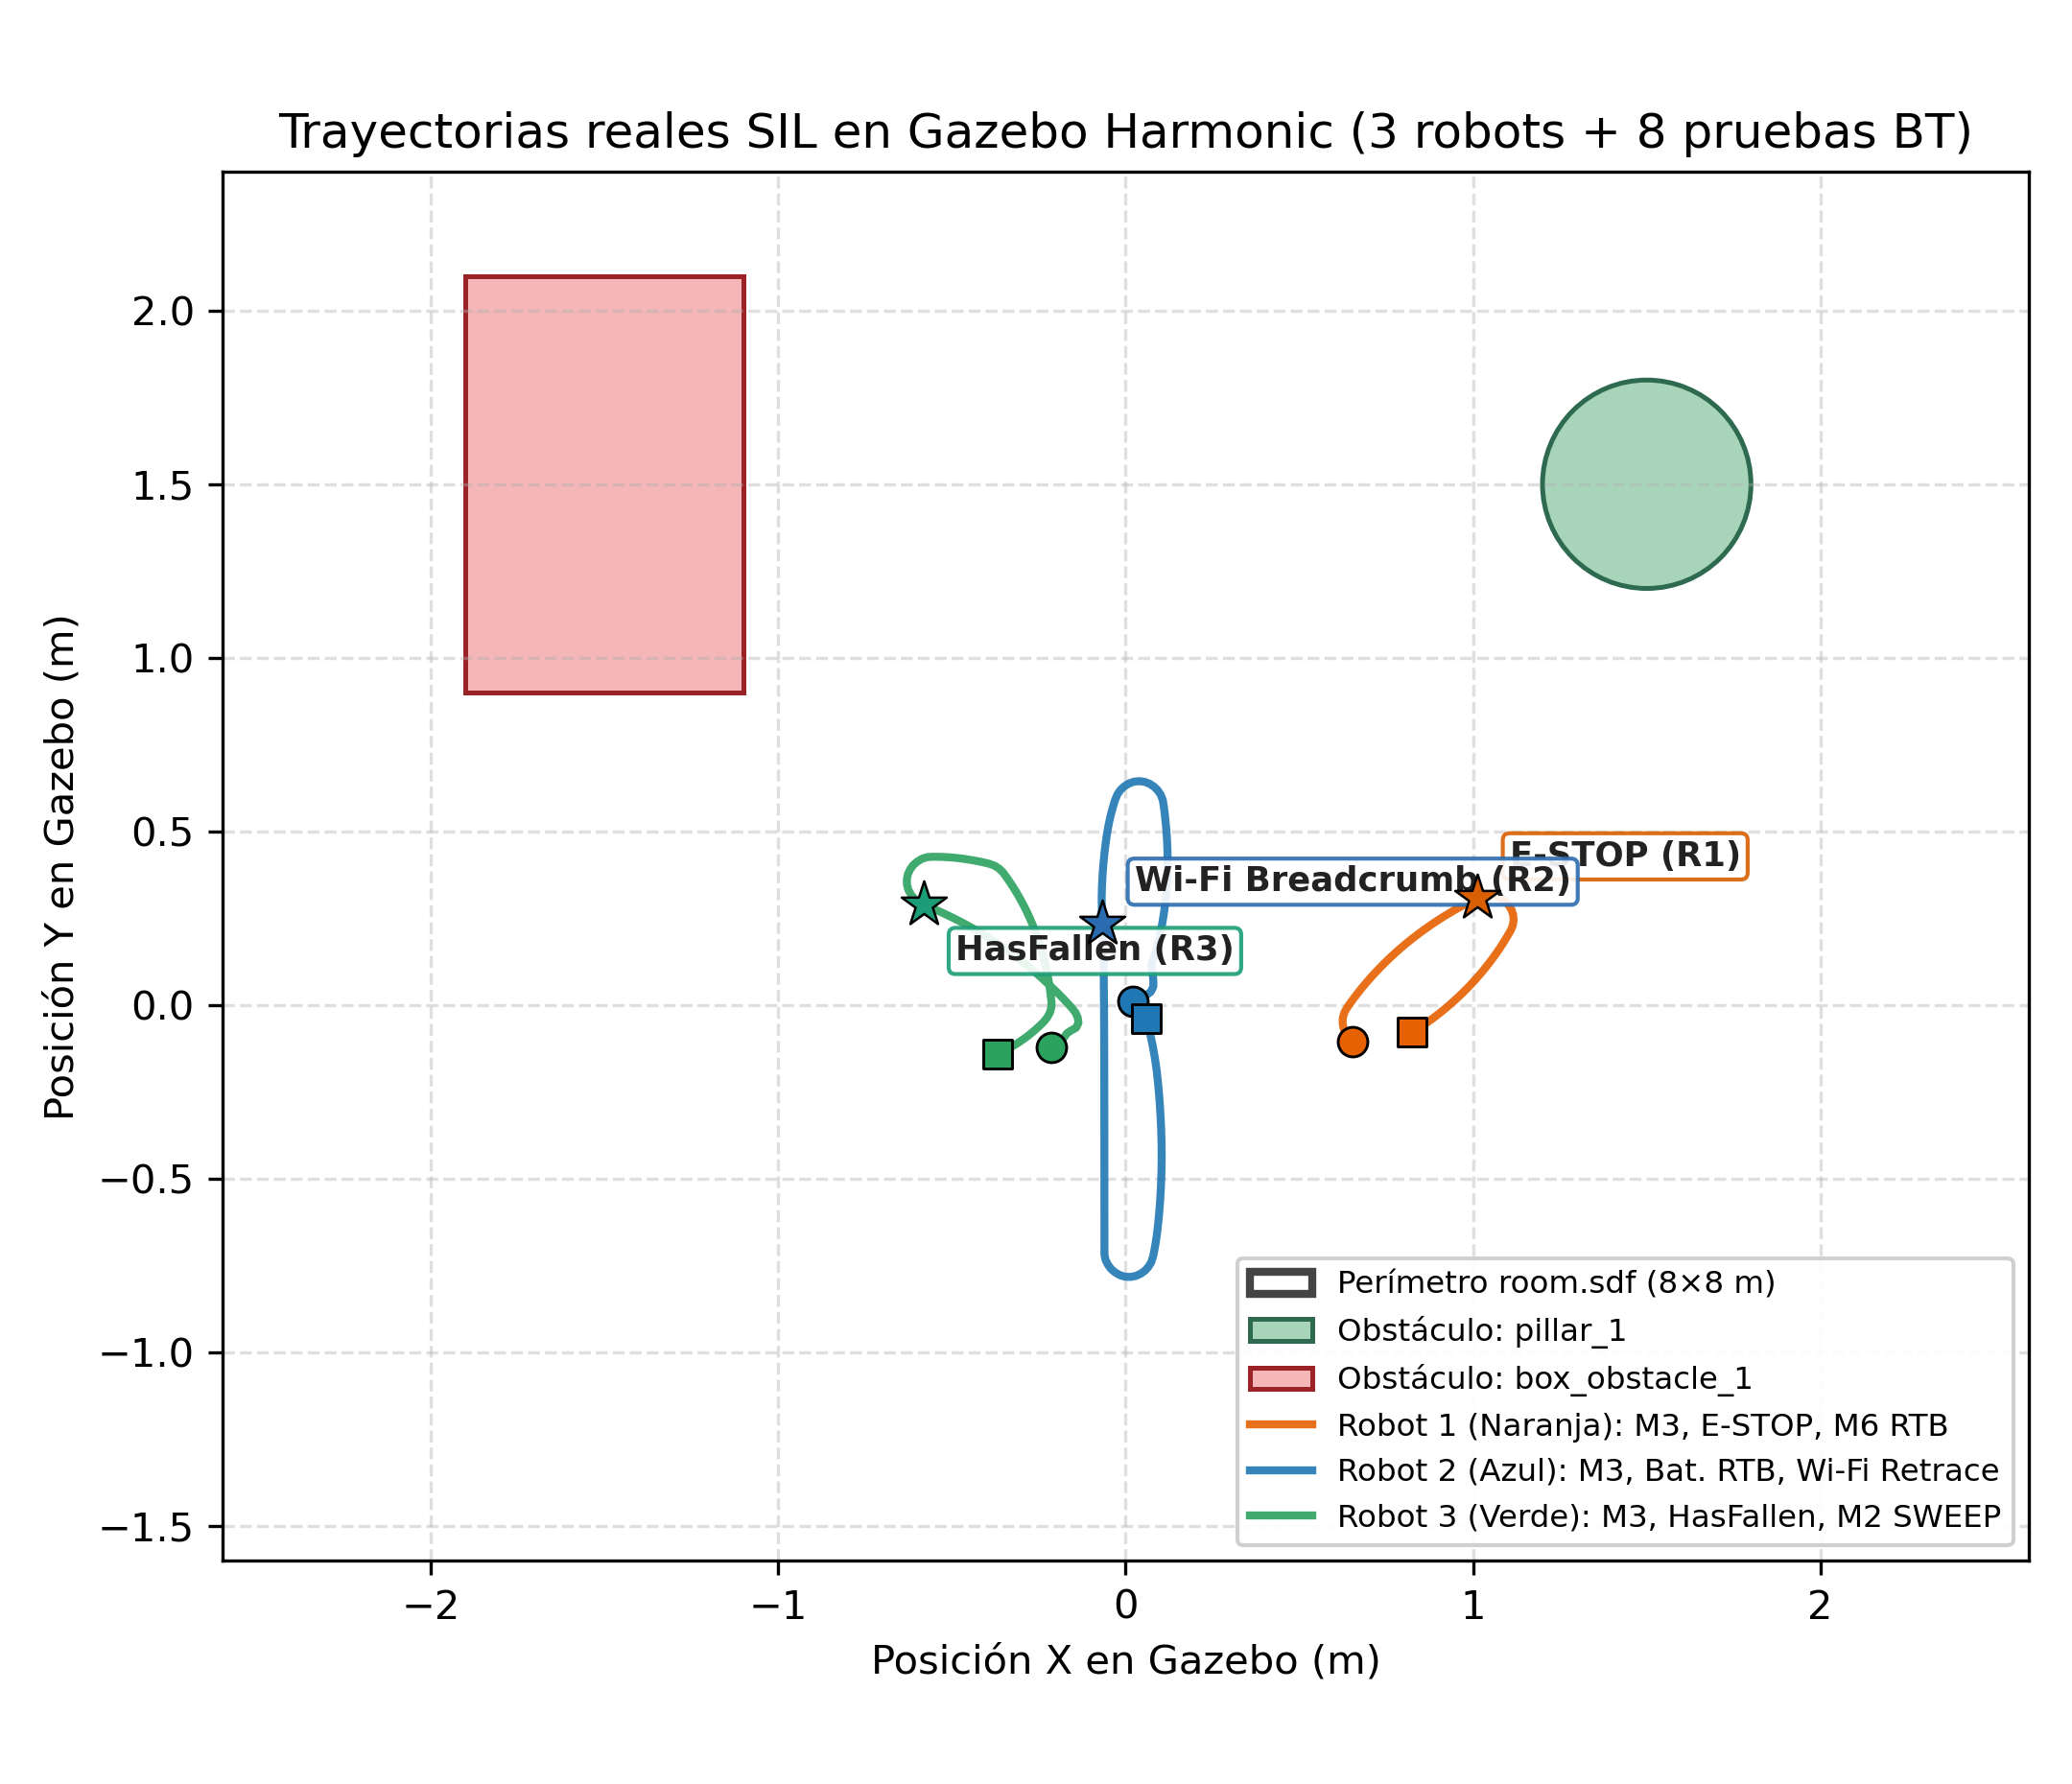
\includegraphics[width=\textwidth]{figuras/sil_trajectories_gazebo.png}
        \caption{Trayectorias reales de odometría y eventos de contingencia durante las 8 pruebas BT.}
        \label{fig:sil_trajectories}
    \end{subfigure}
    \caption{Validación SIL multi-robot sobre Gazebo Harmonic: entorno físico 3D y trayectorias registradas en bucle cerrado.}
    \label{fig:validacion_sil_gazebo}
\end{figure}

\begin{table}[htbp]
    \centering
    \caption{Resultados de la batería automatizada de validación SIL de los Behavior Trees sobre Gazebo Harmonic (3 robots concurrentes).}
    \label{tab:resultados_sil_gazebo}
    \footnotesize
    \begin{tabular}{clcl}
        \toprule
        \textbf{\#} & \textbf{Escenario / Rama evaluada} & \textbf{Estado} & \textbf{Métrica observada en Gazebo} \\
        \midrule
        1 & Conectividad Gazebo $\leftrightarrow$ 3 BTs & \textbf{PASS} & Odometría activa en R1, R2 y R3 \\
        2 & Rama 4: M3 \texttt{GOTO\_POINT} concurrente & \textbf{PASS} & $t=4.9$\,s; error $0.24$--$0.30$\,m \\
        3 & Rama 1: Preempción \texttt{E-STOP} (R1) & \textbf{PASS} & Alerta y parada (\texttt{cmd\_vel}=0) \\
        4 & Rama 1: Vuelco IMU \texttt{HasFallen} $>60^\circ$ (R3) & \textbf{PASS} & Alerta \textit{Rollover/Fallen} y parada \\
        5 & Rama 2: Batería crítica ($10\%$) $\rightarrow$ RTB (R2) & \textbf{PASS} & Retorno al dock ($0.58 \rightarrow 0.25$\,m) \\
        6 & Rama 3: Pérdida Wi-Fi $\rightarrow$ \textit{Retrace} (R2) & \textbf{PASS} & Alejado $0.46$\,m $\rightarrow$ retorno $0.32$\,m \\
        7 & Rama 4: M2 \texttt{SWEEP\_AREA} (3 waypoints, R3) & \textbf{PASS} & $t=10.8$\,s; 3/3 waypoints \\
        8 & Rama 4: M6 \texttt{RTB} explícito + logs Groot2 & \textbf{PASS} & \texttt{START\_RTB}/\texttt{DOCKED} + 3 \texttt{.btlog} \\
        \bottomrule
    \end{tabular}
\end{table}

La Figura~\ref{fig:validacion_sil_gazebo} muestra el entorno 3D en Gazebo Harmonic junto con las trayectorias reales registradas por los tres robots durante la ejecución completa de la batería de pruebas.

\subsection{Incidencias detectadas y corregidas durante la validación SIL}

La ejecución sistemática en Gazebo con el watchdog real de comunicaciones activo (\texttt{simulate\_heartbeat:=false}) permitió detectar y corregir dos defectos relevantes antes del despliegue físico:

\begin{itemize}
    \item \textbf{Reactividad de la Rama~3 (\texttt{Branch3\_Wifi}):} inicialmente modelada como un \texttt{Sequence} plano, impedía abortar el periodo de gracia de 5\,s si el enlace Wi-Fi se recuperaba antes de vencer. Asimismo, cambiar el nodo directamente a \texttt{ReactiveSequence} reiniciaba \texttt{Wait\_WifiGracePeriod} en cada \textit{tick}. La solución definitiva encapsula \texttt{Wait} y \texttt{NavigateToPose} dentro de un subnodo \texttt{Sequence} bajo un \texttt{ReactiveSequence}, logrando cancelación instantánea al recuperar el \textit{heartbeat} sin reiniciar la temporización.
    \item \textbf{Fijación de la miga de pan Wi-Fi (\texttt{last\_known\_wifi\_pose}):} actualizar esta pose desde el callback de odometría durante la ventana de timeout desplazaba el punto seguro hacia la zona sin cobertura. Se vinculó su actualización estrictamente a la recepción efectiva de paquetes en \texttt{/heartbeat}, garantizando que el robot retrocede al último punto con conectividad real confirmada.
\end{itemize}

\chapter{Presupuesto y Planificación}
\label{chap:presupuesto}

Siguiendo la normativa de Trabajos Fin de Titulación de la ETSII -- UPM, este capítulo recoge el análisis económico estimativo del proyecto y el cronograma temporal de ejecución.

\section{Estimación presupuestaria}
\label{sec:presupuesto_costes}

El presupuesto global se desglosa en costes de hardware, herramientas de software y recursos humanos:

\begin{enumerate}
    \item \textbf{Costes de equipamiento hardware:}
    \begin{itemize}
        \item 3$\times$ Robots cuadrúpedos Luwu Dynamics XGO Mini 2S (incluyendo brazos robóticos articulados).
        \item 3$\times$ Sensores LiDAR 2D omnidireccionales y módulos Raspberry Pi Compute Module 5 Lite.
        \item Baterías Li-Ion auxiliares y fuentes de alimentación para banco de pruebas.
    \end{itemize}
    \item \textbf{Costes de software y licencias:}
    \begin{itemize}
        \item El 100\,\% de las herramientas software utilizadas (Ubuntu Linux, ROS 2 Jazzy, Docker Engine, BehaviorTree.CPP v4, Nav2 y compiladores GCC/Clang) se distribuyen bajo licencias libres y de código abierto (\textit{Open Source}), por lo que el coste directo en licencias es de 0,00\,\euro.
    \end{itemize}
    \item \textbf{Costes de personal (Recursos humanos):}
    \begin{itemize}
        \item Dedicación estimada de un Ingeniero de Desarrollo Robótico (horas dedicadas a arquitectura, programación en C++20, simulación, pruebas e integración).
    \end{itemize}
\end{enumerate}

\section{Planificación temporal y cronograma}
\label{sec:cronograma}

\textit{[Sección esquemática: Cronograma de fases y diagrama de Gantt que abarca la revisión bibliográfica, desarrollo del driver, diseño de Behavior Trees, simulación, pruebas en banco y redacción de la memoria].}

\chapter{Conclusiones y Líneas Futuras}
\label{chap:conclusiones}

\section{Conclusiones generales}
\label{sec:conclusiones_gen}

En este Trabajo Fin de Máster se ha desarrollado una arquitectura integral para el control reactivo y la orquestación de una flota de robots cuadrúpedos orientada a operaciones de búsqueda y rescate en el marco del proyecto RASTREO del Centro de Automática y Robótica (CAR CSIC-UPM).

Entre los principales hitos alcanzados destacan:
\begin{itemize}
    \item La sustitución exitosa de la capa de control original por un driver de bajo nivel en C++20 de alto rendimiento y determinista, reduciendo el consumo de cómputo en más de un 95\%.
    \item La articulación de una arquitectura contenerizada en microservicios desacoplados que aísla de forma segura el hardware crítico frente a posibles fallos de navegación.
    \item La formalización de un árbol de comportamiento tolerante a contingencias y estructurado para la ejecución modular de seis misiones operativas clave.
\end{itemize}

\section{Líneas de trabajo futuro}
\label{sec:lineas_futuras}

Como continuación natural a los desarrollos presentados, se proponen las siguientes líneas de trabajo:
\begin{enumerate}
    \item Despliegue y validación en suelo de las misiones de navegación cooperativa Nav2 con los tres perros físicos de forma simultánea.
    \item Incorporación de algoritmos de percepción visual mediante aprendizaje profundo a bordo de la Raspberry Pi CM5 para el reconocimiento automático de víctimas.
    \item Integración de la brigada canina con plataformas humanoides y estaciones de control de campo dentro del ecosistema completo de RASTREO.
\end{enumerate}


% --- Bibliografía ---
\backmatter
% \bibliographystyle{IEEEtran}
% \bibliography{bibliografia}

\end{document}
